% (c) 2016 Daniele Zambelli daniele.zambelli@gmail.com
% (c) 2016 Elisabetta Campana

% \begin{wrapfloat}{figure}{r}{0pt}
% \includegraphics[scale=0.35]{img/fig000_.png}
% \caption{...}
% \label{fig:...}
% \end{wrapfloat}
% 
% \begin{center} \input{\folder lbr/fig000_.pgf} \end{center}

% \subsection{Funzioni, Equazioni e disequazioni con valore assoluto}
% \label{sec:irvalass_}

\chapter{Complementi di algebra}

\section{Equazioni di grado superiore al secondo}
\label{sec:irvalass_supsec}

A questo punto siamo in grado di risolvere equazioni di primo e secondo 
grado. Impareremo ora come comportarci nel caso, più generale, di 
equazioni polinomiali di grado superiore.

\subsection{Equazioni che si possono risolvere tramite scomposizione}
% \label{subsec:irvalass_supsec_scomp}

Pensiamo, ad esempio, di dover risolvere un'equazione polinomiale del 
tipo $P(x)=0$, lo sappiamo già fare? Certo, se possiamo applicare la 
tecnica della scomposizione (raccoglimenti totali e parziali, prodotti 
notevoli, regola di Ruffini...). Scomponiamo il polinomio $P(x)$  
scrivendolo come  prodotto di più polinomi di grado minore e poi, 
mediante la legge dell'annullamento del prodotto, risolviamo le equazioni 
che abbiamo trovato.

Prima di procedere ricordiamo la legge dell'annullamento del prodotto:

\begin{definizione}
Legge dell'annullamento del prodotto: il prodotto di due o più fattori è 
uguale a zero quando almeno uno dei fattori è nullo.   
\end{definizione}

\begin{esempio}
$x^3-4x=0$
\begin{center}
\begin{tabular}{ll}
raccogliamo a fattore comune la $x$: & $x(x^2-4)=0$\\
applichiamo la legge dell'annullamento del prodotto: & $x=0 \sor (x^2-4)=0$\\
risolviamo le due equazioni ottenute: & $x=0 \sor x=\pm 2$
\end{tabular}
\end{center}
\end{esempio}

\begin{esempio}
$3x^3-2x^2-3x+2=0$
\begin{center}
\begin{tabular}{ll}
facciamo un primo raccoglimento parziale: & $3x(x^2-1)-2(x^2-1)=0$\\
raccogliamo a fattore comune la $x$: & $(x^2-1)(3x-2)=0$\\
applichiamo la legge dell'annullamento del prodotto: & $x^2-1=0 \sor 3x-2=0$\\
risolviamo le due equazioni ottenute: $x=\pm 1\sor x=\frac{2}{3}$& 
\end{tabular}
\end{center}
\end{esempio}

\begin{esempio}
$x^4-3x^3+2x^2=0$
\begin{center}
\begin{tabular}{ll}
raccogliamo a fattore comune la $x$: & $x^2(x^2-3x+2)=0$\\
applichiamo la legge dell'annullamento del prodotto: & $x^2=0 \sor x^2-3x+2=0$\\
risolviamo le due equazioni ottenute: & $x=0 \sor x=1 \sor x=2$
\end{tabular}
\end{center}
\end{esempio}

\subsection{Equazioni monomie}

\begin{definizione}[Equazione monomia]
Un'equazione si dice \textbf{monomia} se può essere scritta nella forma:
$$ax^n=0$$      
\end{definizione}

Ricordando che $$x^n=0$$
equivale a $$\underbrace{x\cdot x\cdot x\cdot x \dots \cdot x}_{\text{$n$ 
volte}}=0$$
e per la legge dell'annullamento del prodotto, abbiamo $$x=0 \sor x=0 
\sor x=0 \sor x=0 \sor \cdots \sor x=0 $$
Si può dire quindi che l'equazione $ax^n=0$ ha $n$ soluzioni 
\emph{coincidenti} uguali a 0.

\subsection{Equazioni binomie}

\begin{definizione}[Equazione binomia]
Un'equazione si dice \textbf{binomia} se può essere scritta nella forma:
$$ax^n+b=0$$
dove $n$ è un numero \emph{intero positivo} e $a$ e $b$  \emph{numeri 
reali}  non nulli.  
\end{definizione}

Il numero delle soluzioni dipende da $n$ e dal segno di $a$ e $b$.
Infatti se riscriviamo l'equazione
$$ax^n+b=0$$
e risolviamo rispetto a $x^n$, otteniamo l'equazione equivalente:
$$x^n=-\frac{b}{a}$$

\begin{itemize}
\item se $n$ è \textbf{pari} l'equazione ammette soluzioni reali 
solo se  $-\frac{b}{a}>0$ e le soluzioni saranno date da:
$$x=\pm \sqrt[n]{-\frac{b}{a}}$$
se $-\frac{b}{a}<0$ l'equazione non ammette radici reali in 
quanto non esiste la radice di indice pari di un numero negativo.
\item se $n$ \textbf{dispari} l'equazione ammette sempre 
una sola soluzione reale data da  $$x= \sqrt[n]{-\frac{b}{a}}$$ 
\end{itemize}

\begin{esempio}
$8x^3+1=0$
\begin{center}
\begin{tabular}{ll}
Risolviamo rispetto a $x^3$ e otteniamo l'equazione equivalente: & 
$x^3=-\frac{1}{8}$\\
estraiamo quindi la radice cubica: & $x=\sqrt[3]{-\frac{1}{8}} = -2$
\end{tabular}
\end{center}
\end{esempio}

\begin{esempio}
$4x^2-9=0$
\begin{center}
\begin{tabular}{ll}
Risolviamo rispetto a $x^2$ e otteniamo l'equazione equivalente: & 
$x^2=\frac{9}{4}$\\
le soluzioni di questa equazione sono due: & 
$x=\pm \sqrt{\frac{9}{4}}=\pm\frac{3}{2}$
\end{tabular}
\end{center}
\end{esempio}    

\begin{esempio}
$2x^2 +50=0$

Risolviamo rispetto a $x^2$ e otteniamo l'equazione equivalente: 

$x^2=-\frac{50}{2}=-25$

poiché non ci sono numeri reali che elevati alla seconda diano un risultato 
negativo: 

\emph{L'equazione Non Ha Soluzioni Reali}
\end{esempio}    

\begin{esempio}
$-\frac{2}{3}x^6+2=0$
\begin{center}
\begin{tabular}{ll}
Risolviamo rispetto a $x^6$ e otteniamo l'equazione equivalente: & 
$x^6=-\frac{-2}{-\frac{2}{3}}=3$\\
semplifichiamo: & $x^6=3$\\
le soluzioni di questa equazione sono due: & $x=\pm \sqrt[6]{3}$
\end{tabular}
\end{center}
\end{esempio}

\subsection{Equazioni trinomie particolari}

\begin{definizione}[Equazione trinomia particolare]
Un'equazione si dice \textbf{trinomia particolare} se può essere scritta nella 
forma:
$$ax^{2n}+bx^n+c=0$$
dove $n$ è un numero intero positivo e $a$, $b$ e $c$  numeri reali  non 
nulli. 
\end{definizione}

Possiamo distinguere tre casi:
\begin{itemize}
\item se $n=1$ l'equazione diventa $ax^{2}+bx+c=0$, si riduce 
quindi a un'equazione di secondo grado.
\item se $n=2$ l'equazione diventa $ax^{4}+bx^2+c=0$, con $a$, 
$b$ e $c$ numeri reali  non nulli e viene chiamata \textbf{equazione 
biquadratica}.
\item se $n\geq 2$ le equazioni trinomie si possono ricondurre a 
equazioni di secondo grado tramite una semplice sostituzione:\\
ponendo infatti $x^n=z$ e quindi $x^{2n}=(x^n)^2=z^2$, l'equazione 
di partenza
$$ax^{2n}+bx^n+c=0$$
diventa:
$$az^{2}+bz+c=0$$
ora non resta che risolvere questa equazione, se non troviamo 
soluzioni reali, neppure quella di partenza ammette soluzioni reali, se 
invece ammette soluzioni reali, ad esempio $z_1$ e $z_2$  le soluzioni 
dell'equazione originaria saranno le soluzioni delle due equazioni 
binomie:
\begin{center}
  $x^n=z_1$ e $x^n=z_2$.
\end{center}
\end{itemize}


\begin{comment}
\begin{esempio}

\begin{center}
\begin{tabular}{ll}
: & \\
: & \\
: & 
\end{tabular}
\end{center}
\end{esempio}
\end{comment}

\begin{esempio}
  $x^6+9x^3+8=0$

  Poniamo $x^3=z$, l'equazione diventa: $z^2+9z+8=0$

  Risolviamo questa equazione: 
  $\tonda{z+8}\tonda{z+1}=0 \sRarrow z_1=-8 \sor z_2=-1$

  Ritorniamo ora alla variabile $x$:
  \begin{itemize} [nosep]
    \item $x^3=z_1=-8 \sRarrow x_1=\sqrt[3]{-8}=-2$ 
    \item $x^3=z_2=-1 \sRarrow x_2=\sqrt[3]{-1}=-1$
  \end{itemize}
\end{esempio}

\begin{esempio}
  $x^4+x^2-6=0$
  
  Poniamo $x^2=z$, l'equazione diventa $z^2+z+-6=0$ 
  
  Questa equazione ha soluzioni:
  $\tonda{z+3}\tonda{z-2}=0 \sRarrow z_1=-3 \sor z_2=+2$
  
  Ritorniamo ora alla variabile $x$:
  \begin{itemize} [nosep]
    \item $x^2=z_1 \sRarrow x=-3$ che non ha soluzioni reali
    \item $x^2=z_2 \sRarrow x=+2$ che soluzioni $x_{1,2}=\pm \sqrt[]{2}$
  \end{itemize}
\end{esempio}

\begin{esempio}
  $x^{10}-10x^5+25=0$ 
  
  Poniamo $x^5=z$, l'equazione diventa $z^2-10z+25=0$
  
  Questa equazione ha soluzioni:
  $z_1=5$
  
  Ritorniamo ora alla variabile $x$:
  \begin{itemize} [nosep]
    \item $x^5=z_1 \sRarrow x=5$ che ha soluzione $x=\sqrt[5]{5}$
  \end{itemize}
\end{esempio}


\section{Equazioni e disequazioni irrazionali}
\label{sec:irvalass_irraz}

\subsection{Equazioni irrazionali}

Consideriamo le seguenti equazioni:
\begin{enumerate}
 \item \(\sqrt{x-4} = \dfrac{x-4}{2}\)
 \item \(\sqrt[3]{x^{2}+1} -2=0\)
\end{enumerate}

come si può osservare tali equazioni contengono un radicale nel cui radicando 
compare  l'incognita.
Queste equazioni si dicono irrazionali.

\begin{definizione}[Equazione irrazionale]
 Un'\textbf{equazione irrazionale} è un'equazione algebrica in cui l'incognita 
compare all'interno del radicando di uno o più radicali.
\[\sqrt[n]{A(x)} = B(x)\]
\end{definizione}

Sono quindi equazioni irrazionali: 
\(\sqrt{2x+5} = 3\tonda{x-1}\) \quad e \quad \(\sqrt{2x} = \tonda{3x+4}\)  

mentre non lo sono: \(\sqrt{2} = \tonda{3x-2}\) \quad e \quad 
\(x^2 + \sqrt{3} = 3\) 

Per risolvere un'equazione irrazionale si cerca, tramite opportuni elevamenti a 
potenza, di ricondursi ad un'equazione razionale equivalente.

Ricordiamo che data un'equazione \(A(x)=B(x)\), se eleviamo ambo i membri alla 
\(n\), dove \(n\) è un numero intero positivo, e consideriamo l'equazione 
\(\tonda{(A(x)}^n=\tonda{B(x)}^n\) si possono verificare i seguenti casi:
\begin{itemize}
 \item 
 se n è dispari, essa è equivalente a quella data.
Infatti nel caso n sia un numero dispari è sufficiente elevare entrambi i 
membri 
dell'equazione allo stesso indice, ottenendo  un'equazione razionale che 
ammette 
le stesse soluzioni di quella di partenza.
 \item 
 se n è pari, essa ha come soluzioni, oltre a quelle di \(A(x)=B(x)\), anche 
quelle di \(A(x) = -B(x)\)
Quindi, per risolvere equazioni di questo tipo è sufficiente tenere presente il 
fatto che, elevando ambo i membri alla \(n\) si ottiene un'equazione che 
oltre alle soluzioni di quella data può ammetterne anche altre.
\end{itemize}

\begin{esempio}
 \(sqrt[3]{x^3-x^2-x+25} = x+1\)
 
 elevando ambo i membri al cubo si ottiene: \(x^3-x^2-x+25 = x^3+3x^2+3x+1\)
 
 semplificando si ottiene: 
 \(x^2+x-6=0\) 
 
 che dà come soluzioni:
 \(\tonda{x+3}\tonda{x-2}=0 \sRarrow x_1 = 2 \sor x_2=-3\)
 
 possiamo verificare le soluzioni trovate:
 
 \(\sqrt[3]{2^3-2^2-2+25} = 2+1 \sRarrow \sqrt[3]{8-4-2+25} = 3 \sRarrow 
 \sqrt[3]{27} = 3\)
 
 \(\sqrt[3]{\tonda{-3}^3-\tonda{-3}^2-\tonda{-3}+25} = \tonda{-3}+1 \sRarrow 
 \sqrt[3]{-27-9+3+25} = -2 \sRarrow \sqrt[3]{-8} = -2\)
\end{esempio}

\begin{esempio}
 \(\sqrt{x+4} = 3\)
 
 elevando ambo i membri al quadrato si ottiene: \(x+4 = 9\)
 
 che ha come soluzione: \(x=5\)
 
 possiamo verificare la soluzione:
 \(\sqrt{5+4} = 3 \sRarrow \sqrt{9} = 3\)
\end{esempio}

\begin{esempio}
 \(sqrt{x-3} = x-5\)
 
 elevando ambo i membri al quadrato si ottiene: \(x-3 = x^2-10x+25\)
 
 semplificando si ottiene: \(x^2-11x+28=0\)
 
 che dà come soluzioni:
 \(\tonda{x-7}\tonda{x-4}=0 \sRarrow x_1 = 7 \sor x_2 = 4\)
 
 ora verifichiamo le soluzioni trovate:
 \(\sqrt{7-3} = 7-5 \sRarrow \sqrt{4} = 2\)
 
 \(\sqrt{4-3} = 4-5 \sRarrow \sqrt{1} = -1\)
\end{esempio}

\begin{esempio}
 \(\sqrt{2x+5} = 3 \tonda{x-1}\)
 
 elevando ambo i membri al quadrato si ottiene: \(2x+5 = 9\tonda{x-1}^2\)
 
 semplificando si ottiene: \(2x+5 = 9x^2-18x+9 \sRarrow 9x^2-20x+4=0\)
 
 che dà come soluzioni:
 \(x_{1,2} = \dfrac{10 \mp \sqrt{100-36}}{9} = \dfrac{10 \mp 8}{9} \sRarrow 
 x_1 = \dfrac{2}{9} \sor x_2 = 2\)
 
 ora verifichiamo le soluzioni trovate:
 \(\sqrt{2\cdot 2+5} = 3 \tonda{2-1} \sRarrow \sqrt{9} = 3\) 
 
 \(\sqrt{2\dfrac{2}{9}+5} = 3 \tonda{\dfrac{2}{9}-1} \sRarrow 
   \sqrt{\dfrac{49}{9}} = -\dfrac{7}{9}\)
 
 Quindi \(2\) è una soluzione accettabile, 
 \(\dfrac{2}{9}\) è una soluzione non accettabile (nel senso che è soluzione 
dell'equazione razionale ma non dell'equazione di partenza.
\end{esempio}

% Per riconoscere quali soluzioni siano valide abbiamo due possibilità:
% \begin{enumerate}
%  \item Verificare una per una le soluzioni dell'equazione razionale ottenuta 
% elevando i membri dell'equazione irrazionale e vedere quali di queste 
% verificano anche l'equazione di partenza.
%  \item porre delle condizioni e accettare solo le soluzioni che le soddisfano.
% \end{enumerate}

Quando eleviamo entrambi i membri ad un esponente \emph{pari} otteniamo 
un'equazione che può avere delle soluzioni che non sono soluzioni 
dell'equazione di partenza. Per individuare le soluzioni dell'equazione data 
possiamo verificare, una per una tutte le soluzioni dell'equazione razionale e 
vedere quali di queste sono anche soluzioni di quella irrazionale. Come abbiamo 
fatto negli esempi precedenti.

Un altro metodo consiste nel porre delle condizioni quando eliminiamo le radici 
e accettare poi solo le soluzioni che le soddisfano.

È importante ricordare che:
\begin{enumerate}
 \item la radice di un numero negativo non è un numero reale;
 \item Se esiste, la radice di un numero è sempre positiva.
\end{enumerate}

Perciò, quando passiamo dall'equazione \(\sqrt[n]{A(x)} = B(x)\) 
all'equazione \(A(x) = \tonda{B(x)}^n\)  dobbiamo aggiungere le due 
informazioni che abbiamo perduto in questo passaggio, quindi l'equazione di 
partenza è equivalente al seguente sistema:
\[\sistema{A(x) \geqslant 0 & \text{condizione di realtà} \\
           B(x) \geqslant 0 & \text{condizione di positività} \\
           A(x) = \tonda{B(x)}^n}
\]
Osservando il sistema precedente si può notare che la 
prima condizione può essere tralasciata perché è una conseguenza 
dell'ultima, infatti se \(A(x)\) è uguale a 
\(\tonda{B(x)}^n\) con \(n\) pari, allora senz'altro \(A(x)\) è positivo.

In conclusione l'equazione irrazionale: 
\[\sqrt[n]{A(x)} = B(x)\]
equivale al sistema:
\[\sistema{B(x) \geqslant 0 \\
           A(x) = \tonda{B(x)}^n}
\]

\begin{esempio}
Riprendiamo l'equazione \(\sqrt{2x+5} = 3 \tonda{x-1}\)
 
 è equivalente al sistema: 
\[\sistema{3 \tonda{x-1} \geqslant 0 \\
           x+5 = 9\tonda{x-1}^2}
\]
\(2x+5 = 9\tonda{x-1}^2\)
 
 semplificando si ottiene: 
\[\sistema{x \geqslant 1 \\
           9x^2-20x+4=0}
\]

 che dà come soluzioni:
 \(x_{1,2} = \dfrac{10 \mp \sqrt{100-36}}{9} = \dfrac{10 \mp 8}{9} \sRarrow 
 x_1 = \dfrac{2}{9} \text{ S.N.A } \quad  x_2 = 2 \text{ S.A}\)
 
\end{esempio}

Certi casi semplici possono essere risolti al volo senza particolari calcoli;
tutte le seguenti equazioni irrazionali non hanno soluzioni reali.

\begin{enumerate}
 \item \(\sqrt{5x +8} = -7\) 
 \hfill perché: . . . . . . . . . . . . . . . . . . . . . . . . . . . . . . . .
 \item \(\sqrt{x-4} = -x^2-3\) 
 \hfill perché: . . . . . . . . . . . . . . . . . . . . . . . . . . . . . . . .
 \item \(\sqrt{-x^2} = 9\)  
 \hfill perché: . . . . . . . . . . . . . . . . . . . . . . . . . . . . . . . .
 \item \(\sqrt{4x-5} = -\tonda{x-7}^2\) 
 \hfill perché: . . . . . . . . . . . . . . . . . . . . . . . . . . . . . . . .
 \item \(\sqrt{-\tonda{2x+8}^2} = 14\) 
 \hfill perché: . . . . . . . . . . . . . . . . . . . . . . . . . . . . . . . .
 \item \(\sqrt{-2x^2 + 3x -4} = -x-4\) 
 \hfill perché: . . . . . . . . . . . . . . . . . . . . . . . . . . . . . . . .
\end{enumerate}

\subsection{Disequazioni irrazionali}
\label{sec:irvalass_irrazionali}

Se le disequazioni contengono l'incognita sotto una radice si dicono 
disequazioni \emph{irrazionali}.

Vediamo i casi che si possono presentare.

\subsubsection{Radici con indice dispari}

Le disequazioni irrazionali del tipo:

\[\sqrt[n]{A(x)} \leqslant B(x) \text{ o } \sqrt[n]{A(x)} \geqslant B(x)\]

con \(n\) dispari si risolvono semplicemente elevando ambo i membri della 
disequazione allo stesso indice, ottenendo una disequazione razionale che 
ammette le stesse soluzioni di quella di partenza.

\begin{esempio}
\(\sqrt[3]{-6x^2 +12x +1} \leqslant x -2\)
\begin{center} \begin{tabular}{rl}
elevando ambo i membri al cubo si ottiene: & 
\(-6x^2 +12x +1 \leqslant x^3 -6x^2 +12x -8\)\\
semplificando si ottiene: & \(x^3 -9 \leqslant 0\)\\
che dà come soluzioni: & \(x \leqslant \sqrt[3]{9}\)
\end{tabular} \end{center}
\end{esempio}

\begin{esempio}
\(\sqrt[3]{x^3 -3x +2} > x -1\)
\begin{center} \begin{tabular}{rl}
elevando ambo i membri al cubo si ottiene: & 
\(x^3 -3x +2 > x^3 -3x^2 +3x -1\)\\
semplificando si ottiene: & \(3 \tonda{x -1}^2 > 0\)\\
che dà come soluzioni: & \(\forall x \in \R \sand x \neq 0\) 
\end{tabular} \end{center} 
\end{esempio}

\subsubsection{Radici con indice pari}

In questo testo ci limiteremo al caso \(n=2\), ma il caso più 
generale si affronta in modo analogo.

Le disequazioni irrazionali del tipo:

\[\sqrt[n]{A(x)} \leqslant B(x) \text{ o } \sqrt[n]{A(x)} \geqslant B(x)\]

con \(n\) pari sono equivalenti a un sistema di disequazioni. Possiamo 
distinguere due casi.

\paragraph{Primo caso: \(\sqrt[n]{A(x)} \leqslant B(x)\)}
~

Osservazioni: 
\begin{enumerate} 
 \item Il radicando, deve sempre essere maggiore o uguale a zero. 
Per la condizione di realtà (C.R.) dovrà quindi essere \({A(x)} \leqslant 0\).
 \item Se il radicando è positivo, anche la radice è definita e sarà 
positiva, quindi anche \({B(x)} \leqslant 0\)
 \item Se i membri della disequazione sono entrambi positivi e il primo è 
minore 
del secondo allora anche il quadrato del primo membro deve essere minore del 
quadrato del secondo membro: 
\(\quadra{\sqrt[n]{A(x)}}^2 \leqslant \quadra{B(x)}^2\).
\end{enumerate}
Tradotte in simboli, queste osservazioni producono la seguente equivalenza tra 
la disequazione irrazionale e un sistema di disequazioni razionali:

\[\sqrt[n]{A(x)} \leqslant B(x) \sLRarrow 
  \sistema{A(x) \geqslant 0 \\ 
           B(x) \geqslant 0 \\ 
           A(x) \leqslant \quadra{B(x)}^2}\]

\begin{esempio}
 \(\sqrt{x^2 -4} -4 \leqslant x\)
\begin{center} \begin{tabular}{rl}
riducendo in forma normale: & \(\sqrt{x^2 -4} \leqslant x +4\) \\ [12pt]
equivalente al sistema razionale: &  
\(\sistema{x^2 -4 \geqslant 0 \\ 
           x +4 \geqslant 0 \\ 
           x^2 -4 \leqslant x^2 + 8x +16}\) \\ \\
che si riduce a: &  
\(\sistema{x^2 -4 \geqslant 0 \\ 
           x +4 \geqslant 0 \\ 
           -8x -20 \leqslant 0} \sRarrow 
  \sistema{x \leqslant -2 \sor x \geqslant +2 \\ 
           x \geqslant +4 \\ 
           x \geqslant \frac{5}{2}}\) \\ \\
che dà come soluzioni: & 
\(-\dfrac{5}{2} \leqslant x \leqslant -2 \sor x \geqslant 2\)
\end{tabular} \end{center}
\end{esempio}


\paragraph{Secondo caso: \(\sqrt[n]{A(x)} \geqslant B(x)\)}
~

Abbiamo le seguenti due possibilità: 
\begin{enumerate} 
 \item Se \(B(x) < 0\) per verificare la disequazione basta che la 
radice esista, perché essendo positiva sarà senz'altro maggiore di un numero 
negativo.
 \item Se invece \(B(x)\geqslant 0\) allora il radicando deve 
essere maggiore o uguale al suo quadrato e, in questo caso, verifica anche la 
condizione di esistenza della radice.
\end{enumerate}
Tradotte in simboli, queste osservazioni producono i seguenti due sistemi di 
disequazioni razionali:

\[\sqrt[n]{A(x)} \geqslant B(x) \sLRarrow 
  \sistema{B(x) < 0 \\ 
           A(x) \geqslant 0} \sor 
  \sistema{B(x) \geqslant 0 \\ 
           A(x) \geqslant \quadra{B(x)}^2}\]

\begin{esempio}
 \(\sqrt{4x^2 +3x -1} -2x > -3\)
\begin{center} \begin{tabular}{rl}
riducendo in forma normale: & \(\sqrt{4x^2 +3x -1} > 2x -3\) \\ [12pt]
equivalente all'unione dei sistemi razionali: &  
\(\sistema{2x -3 < 0 \\ 
           4x^2 +3x -1 \geqslant 0} \sor 
  \sistema{2x -3 \geqslant 0 \\ 
           4x^2 +3x -1 > 4x^2 -12x +9}\) \\ \\
che si riduce a: &    
\(\sistema{2x -3 < 0 \\ 
           4x^2 +3x -1 \geqslant 0} \sor 
  \sistema{2x -3 \geqslant 0 \\ 
           15x -10 > 0}\) \\ \\
la soluzione del primo sistema è: & 
\(x \leqslant -1 \sor \dfrac{1}{4} \leqslant x < \dfrac{3}{2}\) \\ \\
la soluzione del secondo sistema è: & 
\(x \geqslant \dfrac{3}{2}\) \\ \\
e l'unione delle soluzioni è: & 
\( x \leqslant -1 \sor x \geqslant -\dfrac{1}{4}\)
\end{tabular} \end{center}
\end{esempio}


\section{Equazioni con valori assoluti}
\label{sec:irvalass_valass}

Per risolvere un'equazione nella quale compare il valore assoluto di qualche 
termine , dobbiamo aver chiaro cosa significa \textbf{valore assoluto di un 
numero reale}.

\subsection{Definizione di valore assoluto}

Si definisce valore assoluto (o modulo) di un numero $x$, e si indica con 
$|x|$, 
una funzione che associa a $x$ un numero reale non negativo. Infatti se $x$ è 
un 
numero reale, il suo valore assoluto è $x$ stesso se $x$ è non negativo, è $-x$ 
se $x$ è negativo.\\
In simboli:
$$|x|=\left\lbrace 
\begin{array}{lcl}
x & \text{se} & x\geq 0 \\
-x & \text{se} & x< 0 \\
\end{array}
\right. 
$$
se riportiamo il numero $x$ sulla retta dei numeri reali, il valore assoluto di 
$x$, $|x|$, non è altro che la distanza del punto che rappresenta $x$, 
dall'origine 0.

\begin{figure}[h]
\begin{center}
\begin{inaccessibleblock}[TODO]
\includegraphics[width=0.8\linewidth]{img/imm1} %[scale=0.35]{img/fig001.png}
\end{inaccessibleblock}
\caption{Retta}
\label{fig:abs_imm1}
\end{center}
\end{figure}

\begin{comment}
%figura:
\begin{figure}[h]
\centering
\includegraphics[width=0.9\linewidth]{imm1}
%\caption{}
\label{fig:imm1}
\end{figure}


% esempio
\begin{esempio}
 
\begin{center} \begin{tabular}{rl}
elevando ambo i membri al cubo si ottiene: & 
 \\
semplificando si ottiene: &  
che dà come soluzioni: &   
\end{tabular} \end{center}
\end{esempio}
\end{comment}

È logico che, per come l'abbiamo definito,\textit{ il valore assoluto di un 
numero reale è sempre non negativo}.

Esempi:
\begin{enumerate}
\item[a.]
$|-2|=-(-2)=2$
\item[b.]
$|+4|=+4$
\item[b.]
$|-2+\sqrt{3}|=-(-2+\sqrt{3})=2-\sqrt{3}$
\end{enumerate} 
Nel caso in cui al posto di $x$ ci fosse una espressione algebrica  $P(x)$ si 
definisce il valore assoluto di $P(x)$, nel seguente modo:
$$|P(x)|=\left\lbrace 
\begin{array}{lcl}
P(x) & \text{se} & P(x)\geq 0 \\
-P(x) & \text{se} & P(x)< 0 \\
\end{array}
\right. 
$$
Vediamo subito alcuni esempi:
\begin{enumerate}
\item
$|x-2|=\left\lbrace 
\begin{array}{lcl}
x-2 & \text{se} & x-2\geq 0 \\
-(x-2) & \text{se} & x-2< 0 \\
\end{array}
\right.
\text{ossia: }
|x-2|=\left\lbrace 
\begin{array}{lcl}
x-2 & \text{se} & x\geq 2 \\
-x+2 & \text{se} & x<2 \\
\end{array}
\right.
$
\item
$|x^2-3x+2|=\left\lbrace 
\begin{array}{lcl}
x^2-3x+2 & \text{se} & x^2-3x+2\geq 0 \\
-(x^2-3x+2) & \text{se} & x^2-3x+2< 0 \\
\end{array}
\right.$
che risolvendo le disequazioni diventa:\\
$
|x^2-3x+2|=\left\lbrace 
\begin{array}{lcl}
x^2-3x+2 & \text{se} & x\leq 1 \vee x\geq 2 \\
-x^2+3x-2 & \text{se} & 1<x<2 \\
\end{array}
\right.
$
\end{enumerate}

\subsection{La funzione ``valore assoluto''}

La funzione $y=|x|$ si chiama funzione valore assoluto ed ha il seguente 
grafico:

\begin{figure}[h]
\begin{center}
\begin{inaccessibleblock}[TODO]
\includegraphics[width=0.6\linewidth]{img/imm2} %[scale=0.35]{img/fig001.png}
\end{inaccessibleblock}
% \caption{Retta}
\label{fig:abs_imm2}
\end{center}
\end{figure}
% \begin{figure}[h]
%         \centering
%         \includegraphics[width=0.9\linewidth]{imm2}
%         %\caption{}
%         \label{fig:imm1}
% \end{figure}

\textbf{Esempio: } Grafico della funzione: $y=|x-2|$:

\begin{figure}[h]
\begin{center}
\begin{inaccessibleblock}[TODO]
\centering
\includegraphics[width=0.6\linewidth]{img/imm3} %[scale=0.35]{img/fig001.png}
\end{inaccessibleblock}
% \caption{Retta}
\label{fig:abs_imm3}
\end{center}
\end{figure}
% \begin{figure}[h]
%         \centering
%         \includegraphics[width=0.9\linewidth]{imm3}
%         %\caption{}
%         \label{fig:imm1}
% \end{figure}

\subsection{Proprietà del valore assoluto}
Il valore assoluto gode delle seguenti proprietà:
\begin{enumerate}
        \item Il valore assoluto della somma di due numeri è \textbf{minore o 
uguale} della somma dei valori assoluti dei due numeri:
        $$|x+y|\leq |x|+|y|, \forall x,y \in \mathbb{R}$$
        Infatti, ad esempio: $|6+(-3)|=3$, mentre $|6|+|-3|=9$, e $3<9$.\\
        Osservazione: questa proprietà prende anche il nome di 
\textbf{disuguaglianza triangolare}.
        \item Il valore assoluto del  prodotto è \textbf{uguale} al prodotto dei 
valori assoluti:
        $$|x\cdot y|=|x|\cdot |y|, \forall x,y \in \mathbb{R}$$
        \item Il valore assoluto del quoziente è \textbf{uguale} al quoziente 
dei valori assoluti:
        $$\left|\frac{x}{y} \right| =\frac{|x|}{|y|}, \forall x \in \mathbb{R}, 
\forall y \in \mathbb{R}_0$$
        \item $$|x|=|y| \leftrightarrow x=\pm y, \forall x,y \in \mathbb{R}$$
        \item $$|x|=|-x|, \forall x \in \mathbb{R}$$
        \item $$|x|^2=x^2, \forall x \in \mathbb{R}$$
        \item $$\sqrt{x^2}=|x|, \forall x \in \mathbb{R}$$
\end{enumerate}

\subsection{Equazioni con il valore assoluto}
Come facciamo a risolvere equazioni nelle quali l'incognita compare all'interno 
di qualche valore assoluto? Vediamo alcuni esempi.\\
\paragraph{1\textdegree~caso}: L'equazione si presenta nella forma:  $|P(x)|=k$

\begin{esempio} 
$|x-5|=-2$, l'equazione non ha soluzione 
perché il valore assoluto di un polinomio è sempre non negativo.
\end{esempio}

\begin{esempio}  
$|x-5|=0$, in questo caso possiamo 
risolvere 
l'equazione ricordando che il valore assoluto di un numero è zero se e solo se 
lo è il numero stesso, quindi $x=0$
\end{esempio}

\begin{esempio}  
$|x-5|=2$, in  questo caso possiamo 
risolvere l'equazione ricordando che  il valore assoluto di un numero è uguale 
ad un numero positivo, $|P(x)|=k>0$, se e solo se $P(x)=\pm k$ (proprietà 4 del 
valore assoluto) l'equazione è equivalente a:
$$x-5=\pm 2$$
che corrisponde a scrivere:
$$x-5= 2 \vee x-5=-2$$
che ha come soluzioni:
$$x=7 \vee x=3$$
\end{esempio}

\textbf{in generale}: se abbiamo un'equazione del tipo: $|P(x)|=k$\\
se $k < 0$  l'equazione non ha alcuna soluzione reale\\
se $k = 0$  l'equazione è equivalente a  $P(x) = 0$\\
se $k > 0$   l'equazione è equivalente a  $P(x)=k \vee P(x)=-k$\\

\begin{esempio} 
$$|2x^2+5x|=0,$$ l'equazione è equivalente a:
$$2x^2+5x=0$$
che ha come soluzioni:
$$x=\dots \vee x=\dots$$
\end{esempio}

\begin{esempio} 
$$|2x^2+5x|=-3,$$ siamo nel caso $k < 0$ 
quindi \emph{l'equazione è impossibile}
\end{esempio}
        
\begin{esempio} 
$$|2x^2+5x|=3,$$ l'equazione è equivalente a:
$$2x^2+5x=3 \vee 2x^2+5x=-3$$
la prima ha soluzioni: $x=\frac{1}{2} \vee x=-3$\\
la seconda ha soluzioni: $x=-\frac{3}{2} \vee x=-1$\\
Pertanto l'insieme delle soluzioni dell'equazione di partenza è: 
$S=\left\lbrace \frac{1}{2},-\frac{3}{2},-1,-3\right\rbrace $
\end{esempio}

\paragraph{2\textdegree~caso}: L'equazione si presenta nella forma:  
$|A(x)|=|B(x)|$\\
Ricordando la proprietà 4 dei valori assoluti tale equazione è equivalente a:
$$A(x)=B(x) \vee A(x)=-B(x)$$

\begin{esempio} $|3x+1|=|x-1|$, l'equazione è equivalente a
$$3x+1=x-1 \vee 3x+1=-x+1$$
la prima ha soluzione: $x=-1$\\
la seconda ha soluzione: $x=0$\\
Pertanto l'insieme delle soluzioni dell'equazione di partenza è: 
$S=\left\lbrace -1,0 \right\rbrace $ 
\end{esempio}
                
\begin{esempio}
E se dovessimo risolvere un'equazione di questo tipo?:
$$|2x-3|=-|x+1|$$
Niente paura, è chiaro che l'equazione è impossibile perché \dots
\end{esempio}

\paragraph{3\textdegree~caso}: L'equazione si presenta nella forma:  
$|A(x)|=B(x)$\\
Cosa dobbiamo fare in questo caso? Dobbiamo semplicemente \textquotedblleft 
sciogliere\textquotedblright il valore assoluto!
Se ricordiamo la definizione di $|A(x)|$ capiamo subito che l'insieme delle 
soluzioni di questa equazione è l'unione degli insiemi delle soluzioni dei 
seguenti sistemi misti:

$$
\left\lbrace 
\begin{array}{l}
A(x)=B(x)\\
A(x)\geq 0\\
\end{array}
\right.
\vee
\left\lbrace 
\begin{array}{l}
-A(x)=B(x)\\
A(x)< 0\\
\end{array}
\right.
$$

Facciamo subito un esempio per capire meglio.

\begin{esempio}  $|2x-1|=x+3$, l'equazione è equivalente a
$$
\left\lbrace 
\begin{array}{l}
2x-1=x+3\\
2x-1\geq 0\\
\end{array}
\right.
\vee
\left\lbrace 
\begin{array}{l}
-(2x-1)=x+3\\
2x-1< 0\\
\end{array}
\right.
$$
il primo sistema ha soluzione: $x=4$\\
il secondo sistema ha soluzione: $x=-\frac{2}{3}$\\
        Pertanto l'insieme delle soluzioni dell'equazione di partenza è: 
$S=\left\lbrace 4,-\frac{2}{3} \right\rbrace $.
\end{esempio}

\subsection{Disequazioni con i valori assoluti}

Vogliamo risolvere alcune semplici disequazioni con valori assoluti, 
riconducibili ai seguenti casi:
$$|P(x)|>k, |P(x)|<k, |P(x)|\geq k, |P(x)|\leq k$$


\paragraph{1\textdegree~caso}: La disequazione si presenta nella forma:  
$|P(x)|\leq k, |P(x)|\geq k$ con $k\leq 0$\\
La soluzione della disequazione $|P(x)|\leq k$ con $k\leq 0$ è molto semplice 
se 
si ricorda che il valore assoluto di una espressione algebrica è sempre non 
negativo e quindi non potrà mai essere minore di un numero negativo. Quindi:

\begin{esempio}  
$|2x-1|\leq -3$, la disequazione è impossibile.
\end{esempio}
\begin{esempio} $|3x-2|\leq 0$, in questo caso poiché il 
valore assoluto di un numero non è mai negativo, la disequazione è verificata 
se e solo se $|3x-2|=0$, cioè $x=\frac{2}{3}$.
\end{esempio}

La disequazione $|P(x)|\geq k$ con $k\leq 0$, sarà invece verificata $\forall x 
\in \mathbb{R}$.

\begin{esempio} $|x^2-1|\geq -3$, la disequazione è 
verificata $\forall x \in \mathbb{R}$.
\end{esempio}

\paragraph{2\textdegree~caso}: La disequazione si presenta nella forma:  
$|P(x)|\leq k$ con $k> 0$\\

\begin{esempio}  $|x-1|\leq 2$, ricordando che il valore 
assoluto di $x$, $|x|$, non è altro che la distanza del punto che rappresenta 
$x$ dall'origine 0 della retta dei numeri reali, allora il valore assoluto di 
un 
numero è $\leq 2$ quando quel numero è compreso fra -2 e +2.\\
        Nella figura sono evidenziati tutti i numeri reali la cui distanza 
dall'origine è $\leq 2$.

\begin{figure}[h]
\begin{center}
\begin{inaccessibleblock}[TODO]
\centering
\includegraphics[width=0.7\linewidth]{img/imm4} %[scale=0.35]{img/fig001.png}
\end{inaccessibleblock}
% \caption{Retta}
\label{fig:abs_imm4}
\end{center}
\end{figure}
%         \begin{figure}[h]
%                 \centering
%                 \includegraphics[width=0.9\linewidth]{imm4}
%                 %\caption{}
%                 \label{fig:imm1}
%         \end{figure}\\

La disequazione precedente è equivalente alla:
$$-2\leq x-1 \leq 2$$
questa doppia disequazione può essere risolta:
\begin{enumerate}
  \item [a)] tramite un sistema:
    $$
    \left\lbrace 
    \begin{array}{l}
    x-1\leq 2\\
    x-1\geq -2\\
    \end{array}
    \right.
    $$
    le cui soluzioni sono:
    $$-1\leq x \leq 3$$
  \item [b)] semplicemente sommando +1 a ciascun anello della catena:
    $$-2+1\leq x-1+1 \leq 2+1$$
    e quindi:
    $$-1\leq x \leq 3.$$
\end{enumerate}
\end{esempio}

\paragraph{3\textdegree~caso}: La disequazione si presenta nella forma:  
$|P(x)|\geq k$ con $k> 0$\\

\begin{esempio} $|x-1|\geq 2$, ricordando che il valore 
assoluto di $x$, $|x|$, non è altro che la distanza del punto che rappresenta 
$x$ dall'origine 0 della retta dei numeri reali, allora il valore assoluto di 
un numero è $\geq 2$ quando quel numero è $\leq -2$ oppure $\geq 2$.\\
        Nella figura sono evidenziati tutti i numeri reali la cui distanza 
dall'origine è $\geq 2$.

\begin{figure}[h]
\begin{center}
\begin{inaccessibleblock}[TODO]
\centering
\includegraphics[width=0.7\linewidth]{img/imm5} %[scale=0.35]{img/fig001.png}
\end{inaccessibleblock}
% \caption{Retta}
\label{fig:abs_imm5}
\end{center}
\end{figure}

%         \begin{figure}[h]
%                 \centering
%                 \includegraphics[width=0.9\linewidth]{imm5}
%                 %\caption{}
%                 \label{fig:imm1}
%         \end{figure}\\
La disequazione precedente è equivalente a:
$$x-1\leq -2 \vee x-1 \geq 2$$
ossia
$$x\leq -1 \vee x\geq 3.$$
\end{esempio}













